\documentclass[12 pt]{article}        	%sets the font to 12 pt and says this is an article (as opposed to book or other documents)
\usepackage{amsfonts, amssymb}					% packages to get the fonts, symbols used in most math
\usepackage{graphicx}
  
%\usepackage{setspace}               		% Together with \doublespacing below allows for doublespacing of the document

\oddsidemargin=-0.5cm                 	% These three commands create the margins required for class
\setlength{\textwidth}{6.5in}         	%
\addtolength{\voffset}{-20pt}        		%
\addtolength{\headsep}{25pt}           	%



\pagestyle{myheadings}                           	% tells LaTeX to allow you to enter information in the heading
\markright{Andrew Mayo\hfill \today \hfill}  
																									% and put the proposition number from the book
                                                	% LaTeX will put your name on the left, the date the paper 
                                                	% is generated in the middle 
                                                 	% and a page number on the right



\newcommand{\eqn}[0]{\begin{array}{rcl}}%begin an aligned equation - allows for aligning = or inequalities.  Always use with $$ $$
\newcommand{\eqnend}[0]{\end{array} }  	%end the aligned equation

%\doublespacing                         	% Together with the package setspace above allows for doublespacing of the document

\newcommand{\qed}[0]{$\square$}        	% make an unfilled square the default for ending a proof

\begin{document}												% end of preamble and beginning of text that will be printed 
\textbf{1 (a)}							% the Proposition number from the book (this one is fictitious)
Prove that $w_0 = \bar{Y} - w_1\bar{X}$: \\ \\
Let 
\begin{displaymath}
  f^\prime(g(w_0))=\frac{\partial L}{\partial \sum_{i=1}^{N}[y^{(i)}-(w_0+w_1x^{(i)})]}
\end{displaymath}
\begin{displaymath}
  g^\prime(w_0)=\frac{\partial \sum_{i=1}^{N}[y^{(i)}-(w_0+w_1x^{(i)})]}{\partial w_0}
\end{displaymath}
then
\begin{displaymath}
  \frac{\partial L}{\partial w_0} = f^\prime(g(w_0)) \cdot g^\prime(w_0) 
\end{displaymath}
\begin{displaymath}
  f^\prime(g(w_0))=\sum_{i=1}^{N}[y^{(i)}-w_0-w_1 x^{(i)}] = N\bar{Y}-Nw_0-Nw_1\bar{X} 
\end{displaymath}
\begin{displaymath}
  g^\prime(w_0)=\sum_{i=1}^{N}-1=-N
\end{displaymath}
\begin{displaymath}
  \frac{\partial L}{\partial w_0} = -N(N\bar{Y}-Nw_0-Nw_1\bar{X})=-N^2\bar{Y}+N^2w_0+N^2w_1\bar{X}
\end{displaymath}
\begin{displaymath}
  0=-N^2\bar{Y}+N^2w_0+N^2w_1\bar{X}
\end{displaymath}
\begin{displaymath}
  w_0=\bar{Y}-w_1\bar{X} \; \square
\end{displaymath}  

Prove that 
\begin{displaymath}
  w_1 = \frac{\frac{1}{N}\sum_{i=1}^{N}x^{(i)}y^{(i)}-\bar{Y}\bar{X}}{\frac{1}{N}\sum_{i=1}^{N}(x^{(i)})^2-\bar{X}^2}
\end{displaymath}
By the chain rule, 
\begin{displaymath}
  \frac{\partial L}{\partial w_1} = \sum_{i=1}^{N}[ -x^{(i)} ( y^{(i)} - (w_0 + w_1 x^{(i)}) ) ]
\end{displaymath}
Setting the partial derivative to 0, we get
\begin{displaymath}
  0 = -\sum_{i=1}^{N}x^{(i)}y^{(i)} + \sum_{i=1}^{N}w_0 x^{(i)} + \sum_{i=1}^{N}[w_1 (x^{(i)})^2]
\end{displaymath}
Since $ w_0 = \bar{Y}-w_1\bar{X} $
\begin{displaymath}
  0 = -\sum_{i=1}^{N}x^{(i)}y^{(i)} + \sum_{i=1}^{N} [ (\bar{Y}-w_1\bar{X}) x^{(i)} ] + \sum_{i=1}^{N}[w_1 (x^{(i)})^2]
\end{displaymath}
\begin{displaymath}
  = -\sum_{i=1}^{N}x^{(i)}y^{(i)} + \bar{Y} \sum_{i=1}^{N} x^{(i)} - \bar{X} w_1 \sum_{i=1}^{N} x^{(i)} + \sum_{i=1}^{N}[w_1 (x^{(i)})^2]
\end{displaymath}
\begin{displaymath}
  w_1 [ \bar{X} \sum_{i=1}^{N} x^{(i)} - \sum_{i=1}^{N}(x^{(i)})^2 ] 
  = -\sum_{i=1}^{N}x^{(i)}y^{(i)} + \bar{Y} \sum_{i=1}^{N} x^{(i)} 
\end{displaymath}
\begin{displaymath}
  w_1 = \frac{ -\sum_{i=1}^{N}x^{(i)}y^{(i)} + \bar{Y} \sum_{i=1}^{N} x^{(i)} } 
  { \bar{X} \sum_{i=1}^{N} x^{(i)} - \sum_{i=1}^{N}(x^{(i)})^2 } 
\end{displaymath}
\begin{displaymath}
  w_1 = \frac{ \sum_{i=1}^{N}x^{(i)}y^{(i)} - N \bar{Y} \bar{X} } 
  { \sum_{i=1}^{N}(x^{(i)})^2 - N \bar{X}^2 } 
\end{displaymath}
\begin{displaymath}
  w_1 = \frac{ \frac{1}{N} \sum_{i=1}^{N}x^{(i)}y^{(i)} - \bar{Y} \bar{X} } 
  { \frac{1}{N} \sum_{i=1}^{N}(x^{(i)})^2 - \bar{X}^2 } \; \square
\end{displaymath} \\ \\

\textbf{1 (b) i.}
Let us first show that if $ \lambda_i > 0 $ for all i, then $ A $ must be PD. \\ \\
For any $ z \neq 0 \in \mathbb{R}^d, z^T A z = z^T (U \Lambda U^T) z $. Let $ y = U^T z $. Then \\
\begin{displaymath} 
  z^T A z = y^T \Lambda y = y_1^2 \lambda_1 + y_2^2 \lambda_2 + ... + y_d^2 \lambda_d
\end{displaymath}
Since $ U $ is an orthogonal matrix, no row or column of $ U $ can consist entirely of zeros, since each row and column must have a norm of 1. The entries of $ y $ can be written as
\begin{displaymath}
  y_1 = u_1^T z, y_2 = u_2^T z, ... , y_d = u_d^T z
\end{displaymath}
Since $ z \neq 0 $, then for at least one $ i = \{1, 2, ..., d\} $, $ y_i \neq 0 $. We have assumed that for all i $ \lambda_i > 0 $. In the expression
\begin{displaymath}
  y_1^2 \lambda_1 + y_2^2 \lambda_2 + ... + y_d^2 \lambda_d
\end{displaymath}
each term will be 0 if $ y_i = 0 $ and greater than 0 if $ y_i \neq 0 $. So 
\begin{displaymath}
  z^T A z > 0 \; \square
\end{displaymath} \\
Now let us show that if $ A $ is PD then for all i $ \lambda_i > 0 $. \\ 
We have it that, for all values of i, $ A u_i = \lambda_i u_i $, where $ u_i $ is a column of $ U $. By multiplying both sides of the equation by $ u_i^T $ on the left, we get
\begin{displaymath}
  u_i^T A u_i = u_i^T \lambda_i u_i 
\end{displaymath}
Because $ A $ is PD and $ u_i \neq 0 \in \mathbb{R}^d $, $ u_i^T A u_i > 0 $. We can write $ u_i^T \lambda_i u_i $ as
\begin{displaymath}
  \lambda_i \sum_{j=1}^{d}u_{ji}^2
\end{displaymath}
where $ u_{ji} $ is entry of $ U $ at the jth row and ith column. If, for any value of i, $ \lambda_i = 0 $, then  
\begin{displaymath}
  \lambda_i \sum_{j=1}^{d}u_{ji}^2 = 0 = u_i^T A u_i 
\end{displaymath}
which would contradict $ A $ being PD. 
Suppose instead that $ \lambda_i < 0 $. 
For all values of i and j, if $ u_{ji} = 0 $ then $ u_{ji}^2 = 0 $, 
and if $ u_{ji} \neq 0 $ then $ u_{ji}^2 > 0 $. 
Since the column vector $ u_i $ is orthonormal, for some value of j, $ u_{ji}^2 > 0 $. In this case,
\begin{displaymath}
  \lambda_i \sum_{j=1}^{d}u_{ji}^2 = u_i^T A u_i < 0
\end{displaymath}
which would also contradict $ A $ being PD. So it must be the case that if $ A $ is PD then, for all values of i,
\begin{displaymath}
  \lambda_i > 0 \; \square
\end{displaymath} \\ \\
\textbf{1 (b) ii.} Let us start with the eigenvalues of $ \Phi^T \Phi + \beta I $. \\
In effect, $ \Phi^T \Phi + \beta I $ differs from $ \Phi^T \Phi $ by having diagonal values shifted by $ \beta $. 
So if, for $ i = \{1, 2, ..., d\} $, the eigenvalues of $ \Phi^T \Phi $ are $ \lambda_i $, then the eigenvalues of $ \Phi^T \Phi + \beta I $ 
are $ \lambda_i + \beta $. We can see this in the following way. 
Let $ A = \Phi^T \Phi $ and $ B = \Phi^T \Phi + \beta I $, and $ \mu_i $ expresses the eigenvalues of $ B $. 
Let $ M $ be the diagonal matrix $ diag(\mu_i) $. Analogously to $ AU = U \Lambda $,
\begin{displaymath}
  BU = U M
\end{displaymath}
Since $ B = A + \beta I $,
\begin{displaymath}
  (A + \beta I) U = U M
\end{displaymath}
\begin{displaymath}
  AU + \beta U = U M
\end{displaymath}
Since $ A U = U \Lambda $,
\begin{displaymath}
  U \Lambda + \beta U = U M
\end{displaymath}
\begin{displaymath}
  U \beta = U M - U \Lambda = U (M - \Lambda)
\end{displaymath}
\begin{displaymath}
  \beta = M - \Lambda \; \square
\end{displaymath}
Therefore, the difference between the diagonal values of $ M $ and $ \Lambda $ is given by $ \beta $,
and the eigenvalues of B (that is, $ \Phi^T \Phi + \beta I $) are given by $ \lambda_i + \beta $. \\ \\
Now let us show that $ A $ and $ B $ have the same eigenvectors. Let $ z $ be an eigenvector of $ B $.
Since the eigenvalues of $ B $ are given by $ \lambda_i + \beta $, we can write
\begin{displaymath}
  Bz = (\lambda_i + \beta) z = \lambda_i z + \beta z
\end{displaymath}
\begin{displaymath}
  A z + \beta I z - \beta I z = \lambda_i z  \\
\end{displaymath}
\begin{displaymath}
  A z = \lambda_i z \; \square
\end{displaymath}
By the definition of eigenvectors and eigenvalues, this means that $ z $ is also an eigenvector of A. 
If $ u_i $ is an eigenvector of $ \Phi^T \Phi $, it is also an eigenvector of $ \Phi^T \Phi + \beta I $. \\ \\
To see that $ \Phi^T \Phi + \beta I $ is PD if $ \beta > 0 $, 
we can first show that $ \Phi^T \Phi $ is PSD. In general, for any matrix $ X $, $ X^T X $ is PSD. 
For any vector $ z \neq 0 \in \mathbb{R}^d $, 
\begin{displaymath}
  z^T (X^T X) z = (X z)^T X z = || X z ||_2^2 \geq 0
\end{displaymath}
From the proof in \textbf{1 (b) i.} we can see that for a PSD matrix, for all values of i, $ \lambda_i \geq 0 $. In this case, if $ \beta > 0 $,
\begin{displaymath}
  \lambda_i + \beta > 0 \; \square
\end{displaymath}
As we have seen, if all the eigenvalues of $ \Phi^T \Phi + \beta I $ are positive, then $ \Phi^T \Phi + \beta I $ is PD. \\ \\
\textbf{1 (c)} We can write $ \sum_{n=1}^{N} log P(y^{(n)} | x^{(n)}) $ as
\begin{displaymath}
  \sum_{n=1}^{N} \{ \mathbb{I}(y^{(n)} = 1) log P(y^{n} = 1 | x^{(n)}) + \mathbb{I}(y^{(n)} = -1) log P(y^{(n)} = -1 | x^{(n)}) \}
\end{displaymath}
For the probabilities of the class labels \{-1, 1\}, 
we can use the standard sigmoid function for logistic regression $ \sigma(w^T x) $
and treat y as $ y \in \{0, 1\} $:
\begin{displaymath}
  \sum_{n=1}^{N} \{
    y^{(n)} log [ \sigma (w^T \phi(x^{(n)}))] + (1 - y^{(n)}) log [1 - \sigma (w^T \phi (x^{(n)}))]^{1 - y^{(n)}} 
  \}
\end{displaymath}
and then set the partial derivative $ f^{\prime}(w) $ to 0,
switching the expression's sign to make it a convex optimization problem:
\begin{displaymath}
  0 = - \sum_{n=1}^{N} \{ 
  y^{(n)} 
  \frac{1}{\sigma [w^T \phi(x^{(n)})]} \sigma [w^T \phi(x^{(n)})] 
  [1 - \sigma (w^T \phi(x^{(n)}))] 
  \phi(x^{(n)})
\end{displaymath}
\begin{displaymath}
  + \: (1 - y^{(n)})
  \frac{1} {1 - \sigma [w^T \phi (x^{(n)})]}
  [- \sigma (w^T \phi(x^{(n)}))]
  [1 - \sigma (w^T \phi(x^{(n)}))]
  \phi(x^{(n)})
  \}
\end{displaymath}
\begin{displaymath}
  0 = - \sum_{n=1}^{N} \{ 
    y^{(n)} [1 - \sigma (w^T \phi(x^{(n)}))] 
  \phi(x^{(n)})
\end{displaymath}
\begin{displaymath}
  - \: (1 - y^{(n)})
  [ \sigma (w^T \phi(x^{(n)}))]
  \phi(x^{(n)})
  \}
\end{displaymath}
\begin{displaymath}
  0 = - \sum_{n=1}^{N} \{
    [ y^{(n)} - \sigma (w^T \phi(x^{(n)})) ] \phi(x^{(n)})
  \}
\end{displaymath}
By setting the partial derivative of expression (4) with respect to $ w $ to 0 we get
\begin{displaymath}
  0 = - \sum_{n=1}^N{} \{
    \frac{exp [ -yw^T \phi(x^{(n)}) ]} {1 + exp[-yw^T \phi(x^{(n)})]} y \phi(x^{(n)})
  \}
\end{displaymath}
\begin{displaymath}
0 = - \sum_{n=1}^N{} \{
  \frac{1} {exp[yw^T \phi(x^{(n)})] + 1} y \phi(x^{(n)})
  \}
\end{displaymath}
If the derivative equation for the negative log likelihood above has $ y = 0 $, 
then the equation becomes
\begin{displaymath}
  0 = - \sum_{n=1}^{N} \{
    [ - \sigma (w^T \phi(x^{(n)})) ] \phi(x^{(n)})
  \}
\end{displaymath}
which is also what we get from the partial derivative equation for the loss function we derived from (4) 
if $ y = -1 $. So maximizing the partial derivative of the log-likelihood function with respect to $ w $ 
is equivalent to minimizing the partial derivative of loss function (4) with respect to $ w $
when $ y = -1 $. If $ y = 1 $, then the derivative equation for the negative log likelihood becomes
\begin{displaymath}
  0 = - \sum_{n=1}^{N} \{
    [ 1 - \sigma (w^T \phi(x^{(n)})) ] \phi(x^{(n)})
  \}
\end{displaymath}
Since $ 1 - \sigma(w^T \phi(x^{(n)})) = \frac{ exp [ - w^T \phi(x^{(n)})) ] } { 1 + exp[ - w^T \phi(x^{(n)})) ] }  $
\begin{displaymath}
0 = - \sum_{n=1}^{N} \{
    \frac{ exp [ - w^T \phi(x^{(n)})) ] } { 1 + exp[ - w^T \phi(x^{(n)})) ] } 
    \phi(x^{(n)})
  \}
\end{displaymath}
We can use the same expression for the partial derivative equation for the loss function in the same way 
if $ y = 1 $: 
\begin{displaymath}
  0 = - \sum_{n=1}^{N} \{
    \frac{1} {exp [w^T \phi(x^{(n)})] + 1 } \phi(x^{(n)}) 
  \}
  =
  - \sum_{n=1}^{N} \{
    \frac{ exp [ - w^T \phi(x^{(n)})) ] } { 1 + exp[ - w^T \phi(x^{(n)})) ] } 
    \phi(x^{(n)})
  \}
\end{displaymath}
Thefore, since $ w $ has the same value at the maximum of the log-likelihood function 
and the minimum of loss function (4) for all values of $ y $, maximizing the log-likelihood 
is equivalent to minimizing this loss function. \\ \\

\textbf{2.1 (b)} 

\begin{figure}[h!]
  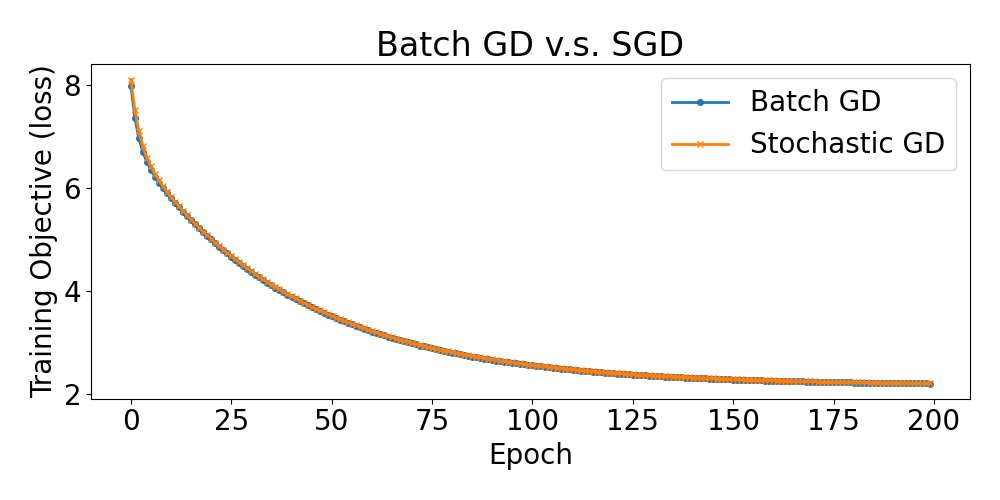
\includegraphics[width=\linewidth]{gd_vs_sgd.png}
\end{figure}

GD took less time (0.00 seconds as opposed to 0.03 seconds for SGD, as measured by the time module)
but SGD showed a lower test objective (2.6796 for SGD vs. 2.7017 for GD). 
SGD updates weights more frequently than GD. Hence it is not surprising
that more frequent computation made SGD take longer. 
In this case, it also seems that the more frequent updates to the weights with SGD 
allowed SGD to minimize the loss on the training set more effectively over a set number
of epochs. \\ \\ \\ \\ \\ \\ \\ \\

\textbf{2.2 (b)}

\begin{figure}[h!]
  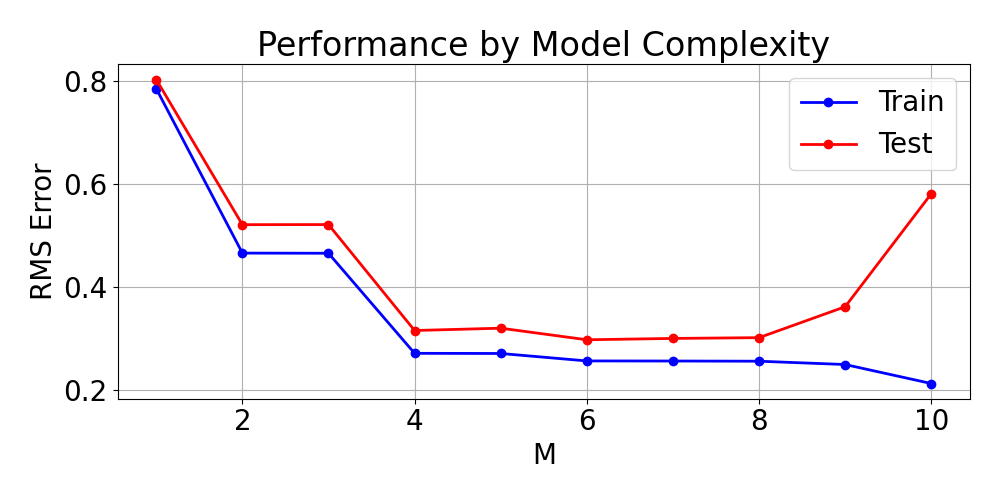
\includegraphics[scale=0.5]{rms_model_size.png}
\end{figure}

\textbf{2.2 (c)}
In the plot in \textbf{2.2 (b)} we see a clear divergance in model performance in the training set vs. the test set at $ M = 8 $, 
that is, with a polynomial of degree 7. For a polynomial of degree 8, it is clearly the case that model performance
on the test set has worsened. I would say that the model with $ M = 6 $, that is, the polynomial of degree 5, 
best fits the data (inclusive of the test set), since we see no improvement in performance
for $ M > 6 $. 
There is clear evidence of overfitting, since in the plot we can see a divergence between training set and test set performance:
the fact that training set performance is still improving while test set performance worsens tells us that the model has overfit the training data.

\newpage \textbf{2.3 (b)}

\begin{figure}[h!]
    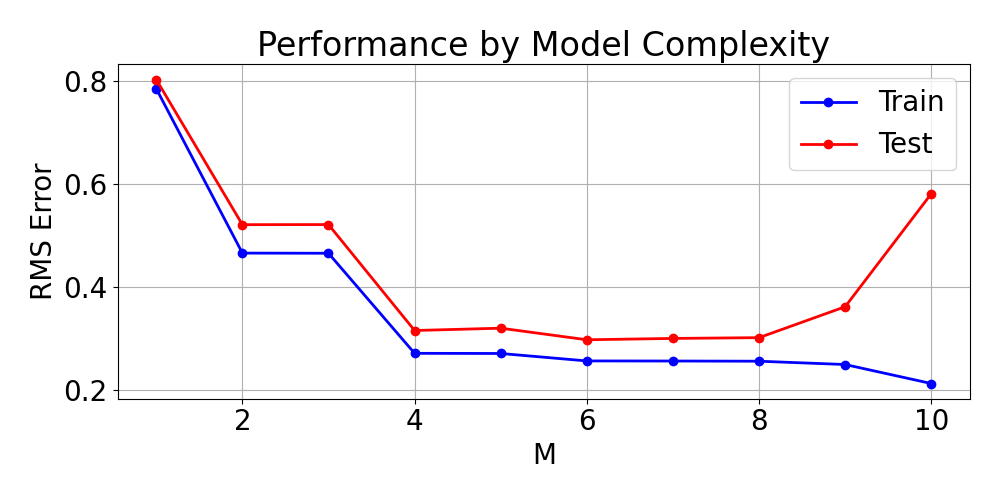
\includegraphics[scale=0.5]{rms_model_size.png}
\end{figure}
\begin{figure}[h!]
    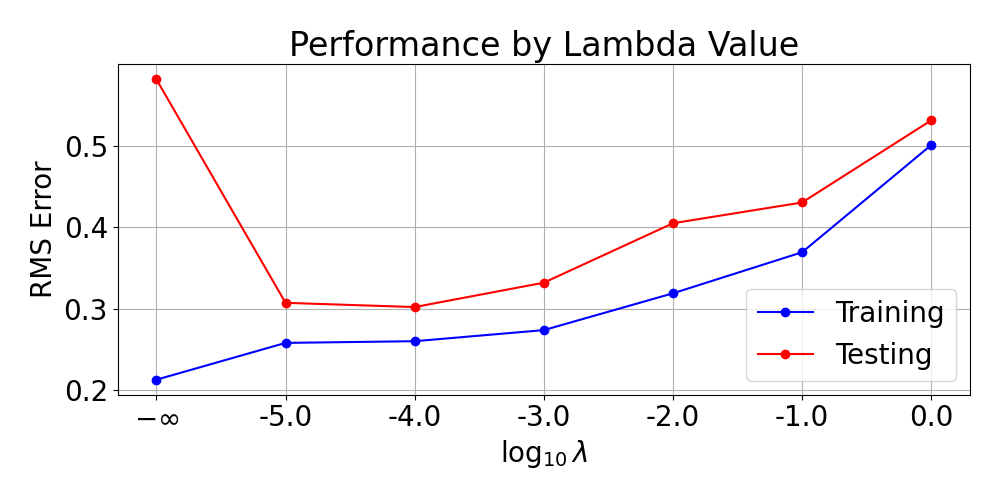
\includegraphics[scale=0.5]{rms_lambda_value.png}
\end{figure}

\textbf{2.3 (c)}
  We see a clear improvement in performance on the test set when we move from $ \lambda = 0 $ (i.e. regression without regularization) 
  to $ \lambda = 0.00001 $, and a slight improve in performance with $ \lambda = 0.0001 $, which seems to be the best value of $ \lambda $ 
  for a ninth degree polynomial.
  We can see this in the way the plot for evaluation on the test set bottoms out at $ \lambda = 0.0001 $. The fact that introducing regularization
  improves performance on the test set but worsens performance on the training set suggests some amount of overfitting.

\textbf{3 (a)} We can write $ E_D(w) = \frac{1}{2} \sum_{i=1}^{N} r^{(i)}(w^T x^{(i)} - y^{(i)})^2 $ as 
\begin{displaymath}
  \sum_{i=1}^{N} frac{r^{(i)}}{2} (w^T x^{(i)} - y^{(i)})^2  
\end{displaymath}
Let $ R = diag(\frac{r^{(i)}}{2}) \in \mathbb{R}^{N \times N}. Now, if we can express this in matrix notation:
{\begin{displaymath}
  (w^T X - y^T) R (w^T X - y^T)^T \; \square  
\end{displaymath}
}


\end{document}

